\section{Introduction}
Exoskeletons and biped robots share many similarities, but exoskeletons have additional constraints. They have to interface with a person who imposes the joint biological limits on the system. The exoskeleton joints should be co-linear with the person and avoid skin irritation. These constraints should be considered when designing a controller for a lower limb exoskeleton. The exoskeleton should comply with human movement to provide a more comfortable fit and make it easier to use.

Lower limb assistive exoskeletons need to be able to navigate different types of terrain found in everyday living. Systems such as, the Rewalk \cite{esquenazi2012rewalk}, the Esko \cite{mertz2012next}, and the Vanderbilt exoskeletons \cite{gasser2017design} have presented promising results; their systems enable people with spinal cord injuries (SCI) and other neurological conditions to stand and walk with assistance \cite{farris2013preliminary}. Both walking and stair climbing are activities of daily living (ADL). Stair climbing is considered a hazardous form of locomotion \cite{HicksLittle2011LowerEJ}  due to the potential for the foot to collide with the stair if the trajectory is incorrect. 

Two fields of interest in lower limb exoskeleton control are the controller's design and the trajectory planner \cite{huang2016optimisation}. These two fields are highly related; the controller produces the torques, while the trajectory generation generates the path for the leg to follow. This work focuses on the generation of the trajectory from the start to the goal, not taking into consideration balance and stability. This research assumes that the goal point is within the exoskeletons support polygon using zero moment point \cite{kajita2003biped}. Exoskeletons directly interface with a person's body and need to  follow the user’s natural joint movement; if this motion does not appropriately match, then there is an excess strain on the person’s joints. The lower level motion controller handles the variation of the mass of the person and the contact dynamics with the environment, while the trajectory generation follows natural motions.

The following paper proposes a learning from demonstration model that uses human motion data. As part of this study, motion capture trials were conducted to collect the necessary data of people of different masses, heights and genders. This data was segmented to extract the motion of climbing the first stair from the floor. The marker on the toe represents the footpath over the step motion while inverse kinematics calculates the joint angles. This structure allows the imitation model to handle various people and stairs of different heights.

The collected data was used to find the general trajectory to climb a stair. Using Gaussian Mixed Model (GMM), the trajectories were encoded into radial basis functions (RBF) placed throughout the data set. The forcing function is found using Gaussian Mixed Regression (GMR), which regresses over the RBFs. This forcing function is used to drive the Dynamic Movement Primitives (DMP) model. This procedure allows for manipulation for temporal, start, and goal manipulation.

\begin{figure} 
    \centering 
    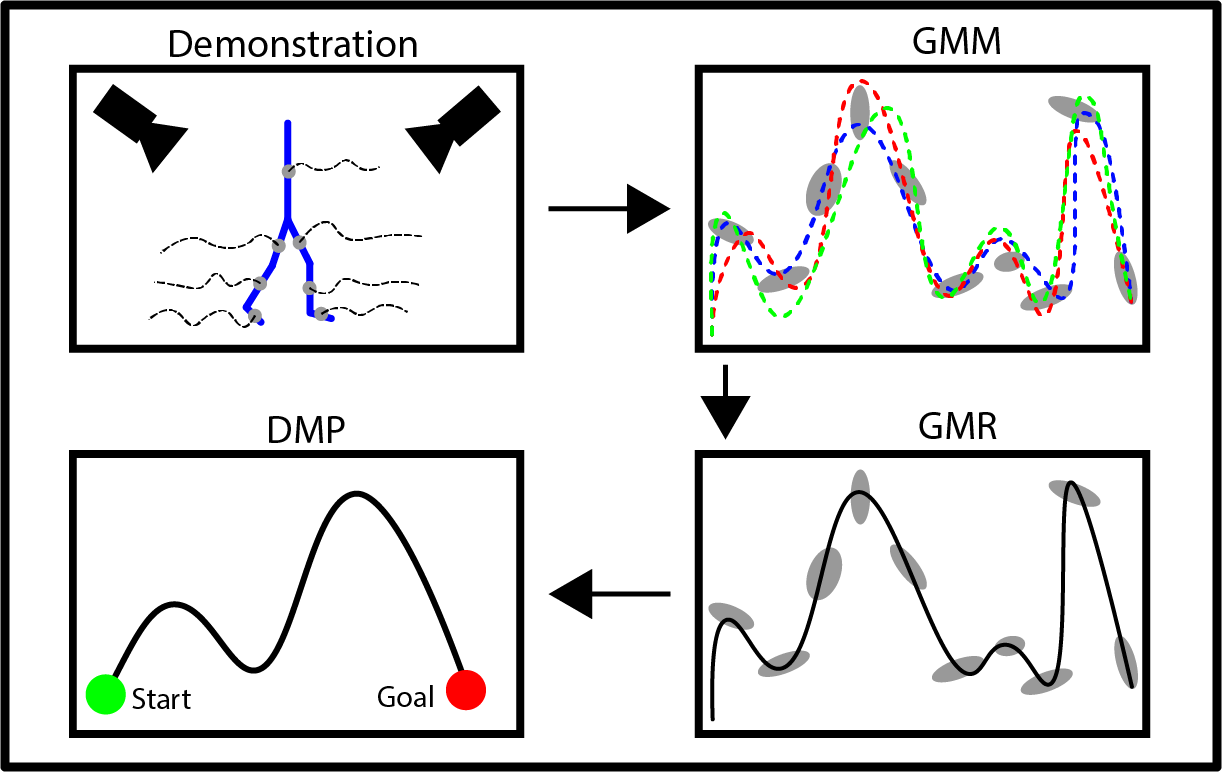
\includegraphics[scale=0.2]{images/demo_figure.png} 
    \caption{Order of operations of the learning process. The data is collected, the demos are encoded, the model is retrieved, then the model is reproduced.} 
    \label{fig:demostation} 
\end{figure} 


This model shows that there is no need to retrain the trajectory for each person and different stair heights. To increase the data in the community, all data used is available online\footnote{\url{https://github.com/WPI-AIM/AIM\_GaitData}}. Increased public data will help the community develop and study human motion.